\documentclass[11pt, oneside]{article}   	% use "amsart" instead of "article" for AMSLaTeX format
\usepackage{geometry}                		% See geometry.pdf to learn the layout options. There are lots.
\geometry{letterpaper}                   		% ... or a4paper or a5paper or ... 
%\geometry{landscape}                		% Activate for for rotated page geometry
%\usepackage[parfill]{parskip}    		% Activate to begin paragraphs with an empty line rather than an indent
\usepackage{graphicx}				% Use pdf, png, jpg, or eps� with pdflatex; use eps in DVI mode
								% TeX will automatically convert eps --> pdf in pdflatex		
\usepackage{amssymb}
\usepackage{amsmath}
\usepackage{parskip}
\usepackage{color}

\title{Fractional power rule}
%\author{The Author}
%\section{}
% \subsection*{R code}
\date{}							% Activate to display a given date or no date

\graphicspath{{/Users/telliott_admin/Dropbox/Tex/png/}}

% \begin{center} 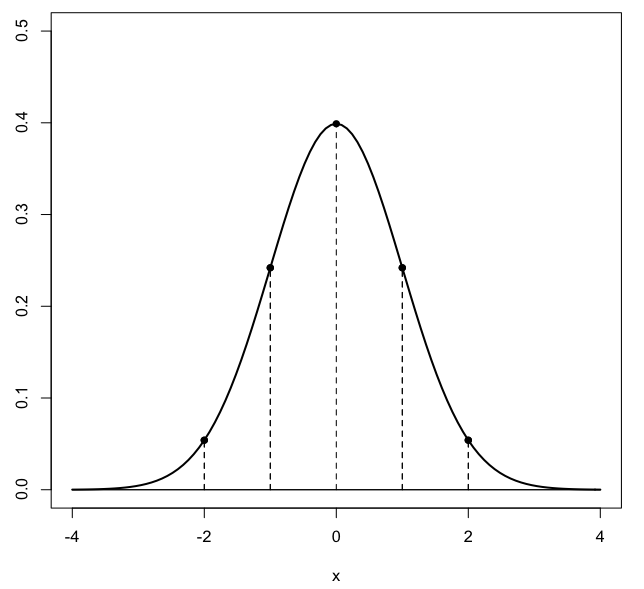
\includegraphics [scale=0.4] {gauss3.png} \end{center}
% \begin{bmatrix} a  &  b \\ c  &  d \end{bmatrix}
% \bigg |_

\begin{document}
\maketitle
\Large
%\noindent
The standard rule for differentiation of powers of $x$ also works for \emph{fractional} powers
\[ \frac{d}{dx} \ x^{p/q} = \frac{p}{q} \ x^{p/q - 1} \]
This is often presented and used without proof.  Here is a simple proof which relies on implicit differentiation.  Write
\[ y = x^{p/q} \]
Now raise both sides to the $q$ power
\[ y^q = x^p \]
Differentiate both sides.  By the chain rule (and differentiating implicitly)
\[ \frac{d}{dx} \ y^{q} = q \ y^{q-1} \ \frac{dy}{dx} \]
The derivative of $x^p$ is as usual, so combining the results we obtain
\[ q \ y^{q-1} \ \frac{dy}{dx} = p \ x^{p-1}\]
Solve for $dy/dx$
\[ \frac{dy}{dx} = \frac{p \ x^{p-1}}{q \ y^{q-1} } \]
Multiply top and bottom by $y$
\[ \frac{dy}{dx} = \frac{p \ x^{p-1} \ y}{q \ y^{q} } \]
Substitute for $y = x^{p/q}$ from above
\[ \frac{dy}{dx} = \frac{p \ x^{p-1} \ x^{p/q}}{q \ y^{q} } \]
Substitute for $y^q = x^p$ from above
\[ \frac{dy}{dx} = \frac{p \ x^{p-1} \ x^{p/q}}{q \ x^p } \]
Simplify
\[ \frac{dy}{dx} = \frac{p}{q} \frac{x^{p/q}}{x } = \frac{p}{q} \ x^{p/q-1} \]





\end{document}  